\documentclass[12pt,letterpaper]{article}
% The usepackage tell LaTeX which packages are needed. As you get better you can add more
% packages for extra functionality
% Percent signs are comments, they will not be read by the renderer.
\usepackage{fullpage}
\usepackage[top=2cm, bottom=2.5cm, left=2.5cm, right=2.5cm]{geometry}
\usepackage{amsmath,amsthm,amsfonts,amssymb,amscd}
\usepackage{lastpage}
\usepackage{enumerate}
\usepackage{fancyhdr}
\usepackage{mathrsfs}
\usepackage{xcolor}
\usepackage{graphicx}
\usepackage{hyperref}
\usepackage[shortlabels]{enumitem}
\usepackage{listings} %for listings of the source code

% Some definitions for using the listing package.
% When we reference 'codegreen', it will be the RGB color defined below.
\definecolor{codegreen}{rgb}{0,0.6,0}
\definecolor{codegray}{rgb}{0.5,0.5,0.5}
\definecolor{codepurple}{rgb}{0.58,0,0.82}
\definecolor{backcolour}{rgb}{0.95,0.95,0.92}
\DeclareUnicodeCharacter{2212}{-}

% Also for the listings, this will make the code listing look like default MATLAB
\lstdefinestyle{mystyle}{
	backgroundcolor=\color{backcolour},   
	commentstyle=\color{codegreen},
	keywordstyle=\color{magenta},
	numberstyle=\tiny\color{codegray},
	stringstyle=\color{codepurple},
	basicstyle=\footnotesize,
	breakatwhitespace=false,         
	breaklines=true,                 
	captionpos=b,                    
	keepspaces=true,                 
	numbers=left,                    
	numbersep=5pt,                  
	showspaces=false,                
	showstringspaces=false,
	showtabs=false,                  
	tabsize=2
}
\lstset{style=mystyle}

\hypersetup{%
  colorlinks=true,
  linkcolor=blue,
  linkbordercolor={0 0 1}
}
 
\setlength{\parindent}{0.0in}
\setlength{\parskip}{0.05in}

\newcommand\course{COMP 521}
\newcommand\hwnumber{3}             
\newcommand\MyName{Zack Humphries}  

\pagestyle{fancyplain}
\headheight 15pt
\lhead{\MyName}
%\lhead{\NetIDa\\\NetIDb}                 % <-- Comment this line out for problem sets (make sure you are person #1)
\chead{\textbf{\Large Homework \hwnumber}}
\rhead{\course\\ \today}
\lfoot{}
\cfoot{}
\rfoot{\small\thepage}
\headsep 1.5em

\begin{document}

%%%%%%%%%%%%%%%%%%%%%%%%%%%%%%%%%%%%%%%%%%%%%%%%%%%%%%%%%%%%%%%%%%%

\section*{Problem}
Calculate finite difference approximation of $u''(x)$ for the function $u(x) = x^2 - cos(10x)$ on the interval $x \in [0.4,1]$. You have to implement the following finite difference approximation:

\begin{equation*}
	\frac{-u_{i+2} + 16u_{i+1}-30u_i+16u_{i-1} - u_{i-2}}{12\Delta x^2}
\end{equation*}

You have to determine the order of accuracy of this approximation. Follow the instructions below.\\

\section*{Instructions}
\begin{enumerate}
	\item You have to work on your solution using the following MATLAB files:
\pagebreak
	\begin{itemize}
		\item \textbf{main.m}
		\lstset{title={main.m}}
        \begin{lstlisting}[language = Matlab]
%% MAIN Program for HW 3
% COMP 521
%
% 1) Calculate the finite difference approximation for the second
%    derivative of a function f(x) on the interval x \in [ 0.4 , 1]
% 2) Determine the order of accuracy of the finite difference
%    approximation using:
%
%   2.1) Absolute error of the midpoint
%   2.2) The root mean square error of the approximation
%   2.3) The infinity norm
%
%   You have to plot the error metrics versus 4 different grid sizes for
%   each case 2.1, 2.2, 2.3. Use loglog plot. Fit the points in the loglog
%   plot to a straight line using polyfit.
%
close all; 
%clear all; 
%clc; 

% Use the following grid sizes
h = [ 0.1 ; 0.05 ; 0.025 ; 0.0125];

% Calculate the number of grid sizes
m = size( h , 1 );

% Specify the Interval
x = [ 0.4 ; 1];

% Initialize an array with the error metrics
errorh = zeros( m , 3 );

% Calculate teh approzimation error for different grid sizes

for i = 1:m
    
    % Apply finite difference approximation
    [ xgrid, Dapprox, aproxlim ] = secderivativeapprox( x, h(i), @Fx );
    
    % Calculate exact solution at the ggrid points
    Dactual = secderivativeactual( xgrid );
    Dactual = Dactual(3:(length(Dactual)-2));       % Because we are ignoring the first 2 and last 2 indexes
    
    % Calculate the error vector
    % Note: Only inlcude the grid points in which tthe approximation was 
    %       computed
    Error = abs( Dapprox - Dactual );
    %Error_rmse = sqrt(Error.*Error/(length(Error)));
    Error_rmse = sqrt(mean((Dapprox-Dactual).^2));
    
    % Calculate the error metrics
    
    % For the midpoint INDEX!!
    impoint = round( ( x(2) - x(1) ) / ( 2*h(i))) + 1;
    
    % Show the midpoint you are using for the current grid to verify
    % that you are using the same x at each h
    fprintf('Midpoint for h=%11.10f is x=%11.10f \n',h(i),xgrid(impoint));
    
    % Save error at midpoint
    errorh(i,1) = Error(impoint-2);
    
    %% This area needs to be coded by you
    % For the rmse
    errorh(i,2) = Error_rmse ;
    
    % For the infinity norm
    errorh(i,3) = max(Error);
    
end

% Plot your results
% Please improve this to make pretty graphs!!

tiledlayout(3,1);

nexttile
loglog(h, errorh(:,1), 'b*'); grid; grid minor;
hold on
loglog(h, errorh(:,1), 'b-')
xlabel('Grid size [h]'); ylabel('|Error_{mid}|');
hold off

nexttile
loglog(h, errorh(:,2), 'r*'); grid; grid minor;
hold on
loglog(h, errorh(:,2), 'r-')
xlabel('Grid size [h]'); ylabel('|Error RSME_{mid}|');
hold off

nexttile
loglog(h, errorh(:,3), 'g*'); grid; grid minor;
hold on
loglog(h, errorh(:,3), 'g-')
xlabel('Grid size [h]'); ylabel('|Error Infinity|');
hold off


% Verify with linear plot fitting
disp(' ' );
% Midpoint Error
Efit = polyfit( log(h), log(errorh(:,1)),1);
disp(['Midpoint: Fit is |E| = ' num2str(Efit(1)) '*h + (' num2str(Efit(2)) ')' ]);

%% You need to code the following parts
% RMSE Error
% Put code here
Efit = polyfit( log(h), log(errorh(:,2)),1) ;
disp(['RMSE: Fit is |E| = ' num2str(Efit(1)) '*h + (' num2str(Efit(2)) ')' ]);

% Infintiy Error
% Put code here
Efit = polyfit( log(h), log(errorh(:,3)),1) ;
disp(['Infinity: Fit is |E| = ' num2str(Efit(1)) '*h + (' num2str(Efit(2)) ')' ]);
\end{lstlisting}
\pagebreak
		\item \textbf{Fx.m}
		\lstset{title={Fx.m}}
        \begin{lstlisting}[language = Matlab]
function foutput = Fx( xin )
% This function evaluates a function f(x) at a given set of inputs x
%
% Inputs:
% xin : x values at which the function is evaluated
%
% Outputs:
% foutput : the results of f(xin)

% Evaluate the function at xin, assign the result to foutput
%
% Write your code here

length_xin = length(xin);
foutput = zeros(1, length_xin);

for i=1:length_xin
    foutput(i) = xin(i)^2-cos(10*xin(i));
end


end\end{lstlisting}
\pagebreak
		\item \textbf{secderivativeactual.m}
		\lstset{title={secderivativeactual.m}}
        \begin{lstlisting}[language = Matlab]
function Dactual = secderivativeactual( xgrid )
% Function that evaluates the exact second derivative of a function f(x)
% on a set of grid points
%
% Inputs:
% xgrid : x points at which the second derivative is evaluated
%
% Outputs:
% Dactual : second derivative values at the grid points


% Write you code here

length_x_grid = length(xgrid);

Dactual = zeros(1, length_x_grid);

for i=1:length_x_grid
    Dactual(i) = 100*cos(10*xgrid(i))+2;
end

end\end{lstlisting}
\pagebreak
		\item \textbf{secderivativeapprox.m}
		\lstset{title={secderivativeapprox.m}}
        \begin{lstlisting}[language = Matlab]
function [ xgrid, Dapprox, aproxlim ] = secderivativeapprox(x, h, Fx )
% This function implements the finite difference approximation of the
% second derivative of a function f(x)
%
% Inputs:
% x   : the X interval
% h   : the step size
% Fx  : handle to the function f(x)
%
% Outputs:
% xgrid     : The grid points in X
% Dapprox   : The finite difference approximation at the grid points
% aproxlim  : The indices of the interval endpoints where the approximation
%             is calculated

% Create the vector with the grid points
xgrid = x(1):h:x(2);

% Set the approximation limits. These limits depend on the finite
% difference approximation you will use.
% Note: In this example we cannot include the first and last endpoints
% into the approximation

firstendpoint = 3;              % Since we rely on ui-2 and u+2, the first usable point is 3
lastendpoint = length(xgrid)-2; % Since we rely on ui-2 and u+2, the last usable point is N-2


% Initialize the array approxlim
% * approxlim(1) : is the index of the first grid point where the finite
%                  difference is calculated
% * aproxlim(2) : is the index of the last grid point where the finite
%                 difference is calculated
%
% Write your code here
aproxlim = [firstendpoint,lastendpoint];





% Initialize the vector that will have the approximation
Dapprox = zeros(1, (lastendpoint-firstendpoint+1)); % +1 because Matlab indexes at 1
% You have to modify this part


% Now calculate the finite difference approximation
%
% Write your code here
x_grid_foutput = Fx(xgrid);         % returns f(x) for all x values on xgrid

length_Dapprox = length(Dapprox);
for i=1:length_Dapprox 
    Dapprox(i) = ((-1*x_grid_foutput(i))+(16*x_grid_foutput(i+1))-(30*x_grid_foutput(i+2))+(16*x_grid_foutput(i+3))+(-1*x_grid_foutput(i+4)))/(12*(h^2));
    % i = u(i-2), i+1 = u(i-1), i+2 = u(i), i+3 = u(i+1), i+4 = u(i+2)
    % Did that because Dapprox and x_grid_foutput are shifted by 2
end

end\end{lstlisting}
	\end{itemize}
\pagebreak
	\item Show the $loglog$ plots with the error metrics versus the grid sizes.
    \begin{figure}[h!]
        \centering
        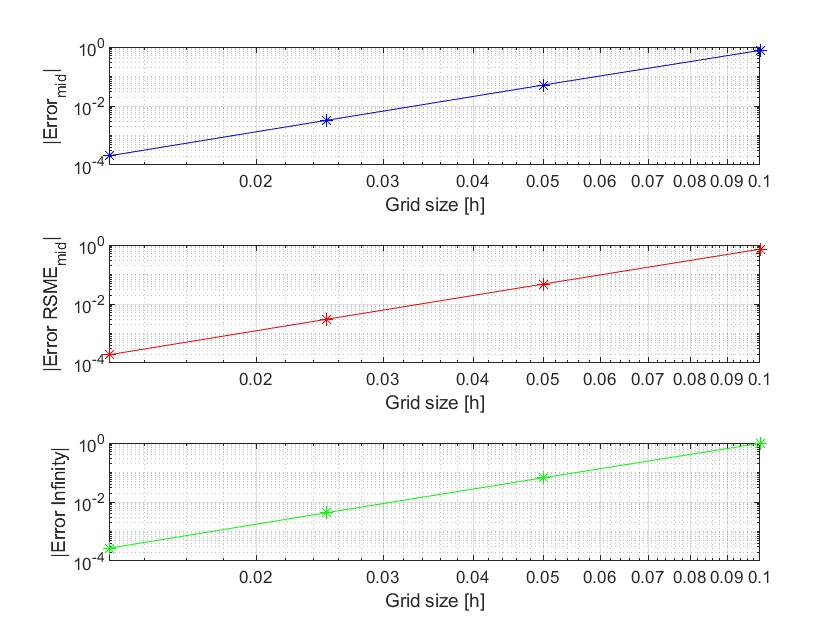
\includegraphics[width=0.75\linewidth]{norm_graphs.jpg}
        \caption{Problem A\: Actual vs Estimate $f''(x)$}\label{fig:Three Norm Graphs}
      \end{figure}  
	\item Fit the $loglog$ plots to a straight line. Use the fit to determine the order of accuracy. Explain.
        
    The output of the program is:
\begin{center}
Midpoint: Fit is $|E| = 3.9596*h + (8.8687)$
\end{center}
\begin{center}
RMSE: Fit is $|E| = 3.9639*h + (8.8112)$
\end{center}
\begin{center}
Infinity: Fit is $|E| = 3.9389*h + (9.0657)$
\end{center}
    Using the coefficients of the three fit equations, the orders of accuracy for all of the metrics are 4.

	\item Discuss the differences from using different metrics. Do they lead to the same conclusion about the order of accuracy?
    
    The order of accuracy is pretty much the same for the taxicab norm, the root mean squared error, and the infinity norm at about 4. This is becuse the finite difference appoximation of $u''(x)$ given is $\mathcal{O}(h^4)$. We don't use the L2-norm of the midpoint because it is sensitive to small changes in the midpoint error. 
\end{enumerate}

\end{document}
